%-------------------------------------------------------------------------------
%	EMPIEZA CAPITULO
%-------------------------------------------------------------------------------

\chapter{Antecedentes al control óptimo}

%-------------------------------------------------------------------------------
%	EMPIEZA SECCION
%-------------------------------------------------------------------------------

    \section{Estabilidad de Lyapunov}

        Dada la siguiente representación de estado:

        \begin{equation} \label{eq:lyap1}
            \frac{dx(t)}{dt} = A x(t) + b u(t)
        \end{equation}

        con $x(0) = x_0  \in \mathbbm{R}^n$.

        \begin{definicion}
            El sistema representado por la ecuación ~\ref{eq:lyap1} es estable si para cada $\epsilon > 0$, existe un $\delta = \delta(\epsilon)$ tal que:

            \begin{equation*}
                ||x_0|| < \delta(\epsilon) \implies  ||x(t)||  < \epsilon \quad \forall t \ge 0
            \end{equation*}

            Si no es estable, decimos que es inestable.

        \end{definicion}

        \begin{marginfigure}
            \centering
            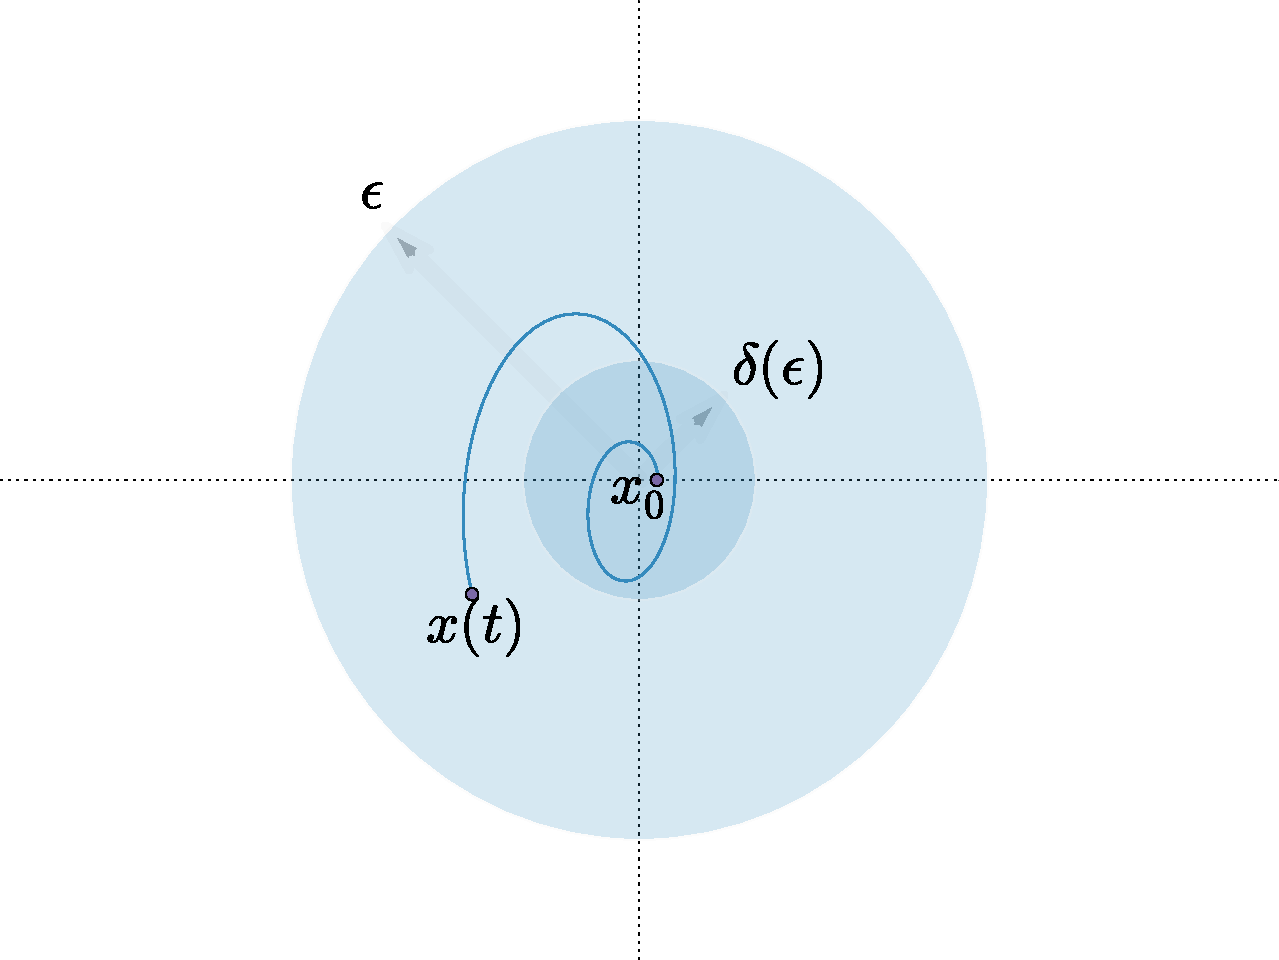
\includegraphics[width=\textwidth]{./imagenes/trayectoriaacotada.pdf}
            \caption{\label{fig:trayectoriaestable}Trayectoria acotada por un limite $\epsilon$.}
        \end{marginfigure}

        \begin{marginfigure}
            \centering
            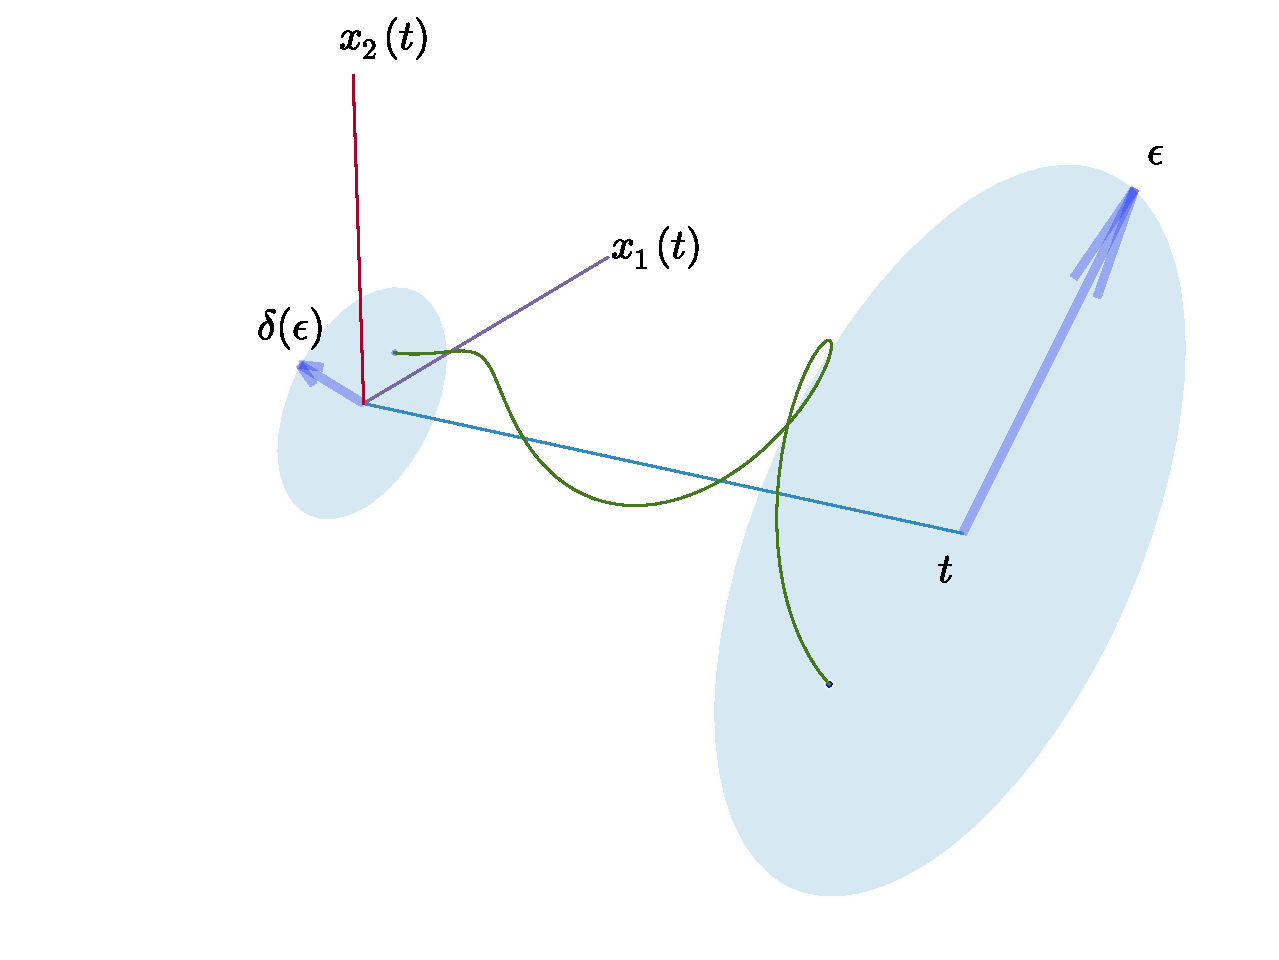
\includegraphics[width=\textwidth]{./imagenes/trayectoriaacotada3d.pdf}
            \caption{\label{fig:trayectoriaestable3d}Trayectoria acotada por un limite $\epsilon$ atraves del tiempo.}
        \end{marginfigure}

        \begin{teorema} \label{te:lyap1}
            Una matriz $A$ es Hurwitz estable, es decir $\Re{\{ \lambda(A) \}} < 0$, si y solo si para cualquier matriz simetrica definida positiva dada, $Q$, existe una matriz simétrica definida positiva, $P$, que satisface:

            \begin{equation}
                A^T P + P A = -Q
            \end{equation}
        \end{teorema}

        \begin{nota}
            \tarea{Resumen de matrices Hermitianas de Introduction to Matrix Computations - G.W. Stewart Cap. 4 y 6}
            Una matriz $H \in \mathbbm{C}^{n\times n}$, se dice Hermitiana si su transpuesta conjugada es ella misma, $H^* = H$.
            Si $H \in \mathbbm{R}^{n \times n}$, se dice simétrica si su transpuesta es ella misma, $H^T = H$.

            De estas matrices, podemos notar ciertas propiedades:

            \begin{enumerate}
                \item Todos sus valores propios son reales.
                \item Cuando los valores propios de $H$ son todos positivos o negativos, se dice que $H$ es definida positiva o negativa, y se escribe $H > 0$ o $H < 0$ respectivamente.
                \item Cuando los valores propios de $H$ son todos no negativos o no positivos, se dice que $H$ es semidefinida positiva o semidefinida negativa y se escribe $H \ge 0$ o $H \le 0$ respectivamente.
                \item Desigualdad de Raleigh

                Dada $H$ Hermitiana:

                \begin{equation*}
                    \lambda_{min}(H) x^* x \le x^* H x \le \lambda_{max}(H) x^*x \quad \forall x \in \mathbbm{C}^n
                \end{equation*}

                Dada $H$ simétrica:

                \begin{equation*}
                    \lambda_{min}(H) x^T x \le x^T H x \le \lambda_{max}(H) x^T x \quad \forall x \in \mathbbm{C}^n
                \end{equation*}
                \item $H$ es semidefinida positiva, si y solo si, puede escribirse de la forma factorizada:

                \begin{equation*}
                    H = G^* G
                \end{equation*}

                para alguna matriz $G$, conocida como raiz cuadrada de $H$, tambien denotada por $H_{\sfrac{1}{2}}$, $\sqrt{H}$, $H^{\sfrac{1}{2}}$, por lo que la factorización queda como sigue:

                \begin{equation*}
                    H = H_{\sfrac{1}{2}}^* H_{\sfrac{1}{2}}
                \end{equation*}

                Cuando $H$ es definida positiva, $H_{\sfrac{1}{2}}$ es una matriz de rango pleno.
            \end{enumerate}
        \end{nota}

        \begin{proof}
            \tarea{Resumen de estabilidad de Lyapunov de Linear Systems - Thomas Kailath Cap. 2.6}
            Sea la función de Lyapunov:

            \begin{equation} \label{eq:lyap2}
                V(x(t)) = x^T P x(t) \quad \forall t \ge 0
            \end{equation}

            con $P = P^T > 0$.

            Derivando a la ecuación ~\ref{eq:lyap2} con respecto del tiempo, a lo largo de las trayectorias solución de la ecuación ~\ref{eq:lyap1}, con $u = 0$, se tiene:

            \begin{eqnarray} \label{eq:lyap3}
                \frac{dV}{dt} & = & \frac{dx(t)}{dt}^T P x(t) + x^T(t) P \frac{dx(t)}{dt} \nonumber \\
                & = & x^T(t) A^T P x(t) + x^T(t) P A x(t) \nonumber \\
                & = & x^T(t) \left( A^T P + P A \right) x(t) \nonumber \\
                & = & -x^T(t) Q x(t)
            \end{eqnarray}

            Por otro lado, de la ecuación ~\ref{eq:lyap2} se tiene:

            \begin{equation*}
                \lambda_{min}(P) x^T(t) x(t) \le V(x(t)) \le \lambda_{max}(P) x^T(t) x(t)
            \end{equation*}

            por lo que:

            \begin{equation} \label{eq:lyap4}
                0 \le \frac{V(x(t))}{\lambda_{min}(P)} \le x^T(t) x(t) \le \frac{V(x(t))}{\lambda_{max}(P)}
            \end{equation}

            Entonces, de las ecuaciones ~\ref{eq:lyap3} y ~\ref{eq:lyap4} se obtiene:

            \begin{equation} \label{eq:lyap5}
                \frac{dV(x(t))}{dt} \le - \frac{\lambda_{min}(Q)}{\lambda_{max}(P)} V(x(t))
            \end{equation}

            De manera análoga

            \begin{equation*}
                \lambda_{min}(Q) x^T(t) x(t) \le x^T(t) Q x(t) \le \lambda_{max}(Q) x^T(t) x(t)
            \end{equation*}

            Si integramos la ecuación ~\ref{eq:lyap5} tendremos:

            \begin{equation*}
                \int_{0}^{t}\frac{dV(x(\tau))}{d\tau} d\tau \le - \frac{\lambda_{min}(Q)}{\lambda_{max}(P)} \int_{0}^{t} V(x(\tau)) d\tau
            \end{equation*}

            para lo cual necesitamos el lema de Bellman - Grönwall.\tarea{Feedback Systems - Input/Output Properties - Desoer, Vidyasagar Ap. E}
            \begin{equation*}
                u(t) \le c + \int_0^t K(\tau) u(\tau) d\tau \implies u(t) \le c \exp{\left( \int_0^t K(\tau) d\tau \right)} \quad \forall t \ge 0
            \end{equation*}

            por lo tanto, podemos ver que:

            \begin{equation}
                V(x(t)) \le V(x(0)) - \frac{\lambda_{min}(Q)}{\lambda_{max}(P)} \int_0^t V(x(\tau)) d\tau
            \end{equation}

            y aplicando el lema de Bellman - Grönwall aqui:

            \begin{equation} \label{eq:lyap6}
                V(x(t)) \le V(x(0)) \exp{- \frac{\lambda_{min}(Q)}{\lambda_{max}(P)} t} \quad \forall t \ge 0
            \end{equation}

            de la ecuación ~\ref{eq:lyap4} y ~\ref{eq:lyap6}, obtenemos finalmente:

            \begin{equation*}
                0 \le x^T(t)x(t) \le \frac{\lambda_{max}(P)}{\lambda_{min}(P)} x^T(0)x(0) \exp{\left( - \frac{\lambda_{min}(Q)}{\lambda_{max}(P)} t \right)}
            \end{equation*}

            es decir:

            \begin{equation*}
                ||x(t)||^2 \le \frac{\lambda_{max}(P)}{\lambda_{min}(P)} ||x(0)||^2 \exp{\left( - \frac{\lambda_{min}(Q)}{\lambda_{max}(P)} t \right)}
            \end{equation*}

            Dado que $A$ es Hurwitz estable tenemos que $\Re{\lambda(A)} < 0$, sea la siguiente matriz definida positiva:

            \begin{equation*}
                P = \int_0^{\infty} \exp{(A^Tt)} Q \exp(At) dt
            \end{equation*}

            con $Q = Q^T > 0$. Entonces tendremos:

            \begin{eqnarray*}
                A^T P + P A & = & \int_0^{\infty} \left( A^T \exp{(A^T t)} Q \exp{(At)} + \exp{(A^T t)} Q \exp{(At)} A \right) dt \\
                & = & \int_0^{\infty} \frac{d}{dt} \left( \exp{(A^T t)} Q \exp{(At)} \right) dt \\
                & = & \left. \exp{(A^T t)} Q \exp{(At)} \right|_0^{\infty} \\
                & = & \lim_{t \to \infty} \exp{(A^T t)} Q \exp{(At)} - \exp{(A^T \cdot 0)} Q \exp{(A \cdot 0)} \\
                & = & 0 - Q = - Q
            \end{eqnarray*}
        \end{proof}

        \begin{marginfigure}
            \centering
            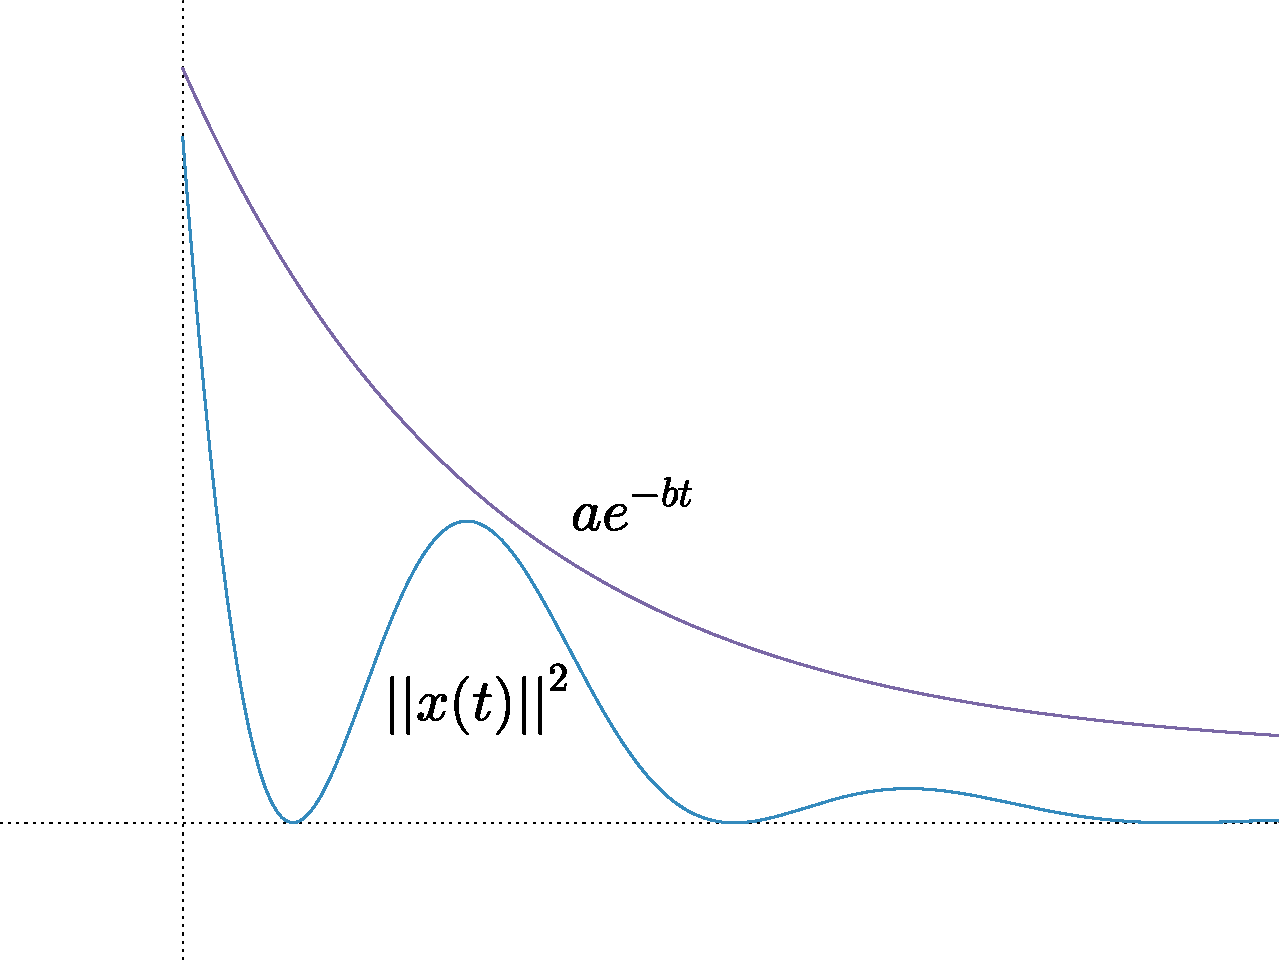
\includegraphics[width=\textwidth]{./imagenes/trayectoria.pdf}
            \caption{\label{fig:trayectoria}Solución exponencialmente estable.}
        \end{marginfigure}

        \begin{lema}
            La ecuación matricial $A X = X B$, tiene unicamente la solución trivial, $X=0$, si y solo si, $A$ y $B$ no tienen valores propios en común, es decir:
            \begin{equation*}
                \sigma(A) \cap \sigma(B) \ne \emptyset
            \end{equation*}
        \end{lema}

        \begin{proof}
            \tarea{Buscar demostración en The Theory of Matrices - F.R. Gantmacher, Vol 1, Cap. 8}
        \end{proof}

        \begin{corolario} \label{co:lyap1}
            En el teorema~\ref{te:lyap1} se puede elegir a $Q$ como una matriz semidefinida positiva, $Q \ge 0$, bajo la condición inicial de que $x^T(t) Q x(t)$ no sea identicamente nula a lo largo de cualquier trayectoria no nula, solución de:

            \begin{equation*}
                \frac{d x(t)}{dt} = A x(t)
            \end{equation*}

            El requerimiento de este corolario se reduce a la condición de que el par $(Q_{\sfrac{1}{2}}, A)$ sea observable:

            \begin{equation*}
                Q \ge 0 \exists Q_{\sfrac{1}{2}} \text{ tal que } Q = Q_{\sfrac{1}{2}}^T Q_{\sfrac{1}{2}}
            \end{equation*}
        \end{corolario}

        \begin{corolario} \label{co:lyap2}
            Si $A$ es una matriz Hurwitz estable entonces la ecuación de Lyapunov, $A^T P + P A = -Q$, tiene una única solución para cada $Q$.
        \end{corolario}

        \begin{proof}
            Suponga que existen dos soluciones, $P_1$ y $P_2$, de la ecuación de Lyapunov, es decir:

            \begin{eqnarray*}
                A^T P_1 + P_1 A & = & -Q \\
                A^T P_2 + P_2 A & = & -Q
            \end{eqnarray*}

            lo cual implica:

            \begin{eqnarray*}
                A^T (P_2 - P_1) + (P_2 - P_1) A & = & 0 \\
                A^T (P_2 - P_1) - (P_2 - P_1) (-A) & = & 0 \\
            \end{eqnarray*}

            pero sabemos que el espectro de una matriz, no cambia debido a la transposición, $\sigma(A^T) = \sigma(A)$, y por otro lado tenemos que la matriz $A$ es Hurwitz estable, es decir $\Re{\left\{ \lambda(A)\right\}} < 0$, lo cual implica que:

            \begin{equation*}
                \Re{\left\{ \lambda(-A) \right\}} > 0
            \end{equation*}

            por lo que podemos concluir que:

            \begin{equation*}
                \sigma(A^T) \cap \sigma(-A) = \emptyset
            \end{equation*}

            por lo tanto, solo hay una solución y es la trivial.
        \end{proof}

%-------------------------------------------------------------------------------
%	EMPIEZA SECCION
%-------------------------------------------------------------------------------

    \newpage
    \section{Introducción a la optimización de funcionales}

        El problema que tratamos de resolver es el siguiente; determinar $v(t)$, tal que la siguiente ecuación:

        \begin{equation} \label{eq:opfun1}
            J(v(t), v'(t)) = \int_{t_1}^{t_2} f_1(v(t), v'(t), t) dt
        \end{equation}

        sea un extremo.

        Primero definamos una función de vecindad $v(t) \to v(\alpha, t)$ tal que si $\alpha = 0 \implies v^* = v(0, t) = v(t)$, es decir, $v^*$ es la función que extremiza a $J(v(t), v'(t))$.

        Proponemos una solución en forma lineal:

        \begin{equation}
            v(\alpha, t) = v(0, t) + \alpha \eta(t)
        \end{equation}

        pero $v(t)$ y $u(t)$ deben ser idénticos en los puntos extremos.

        \begin{marginfigure}
            \centering
            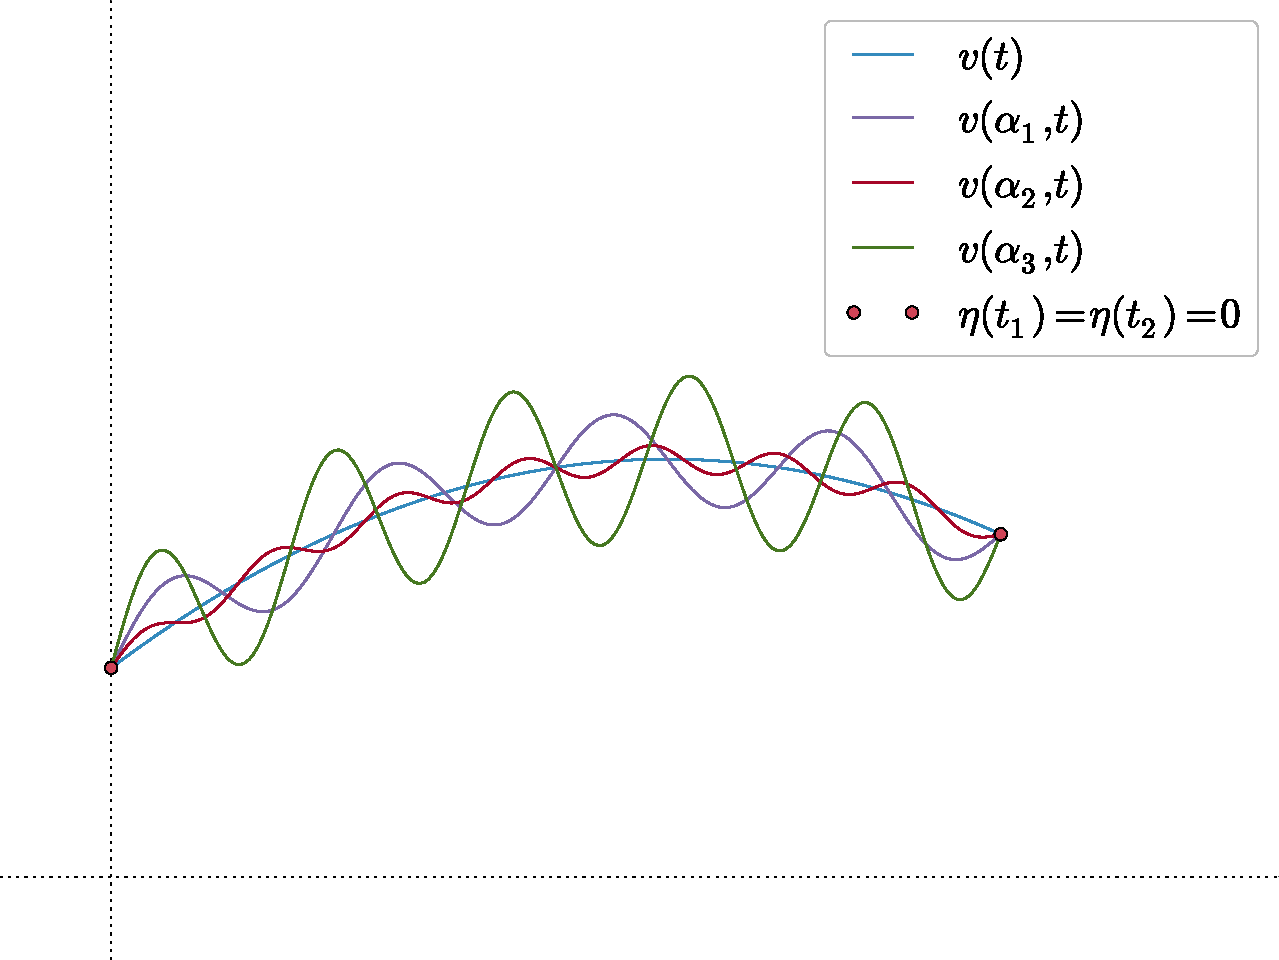
\includegraphics[width=\textwidth]{./imagenes/trayectorias.pdf}
            \caption{\label{fig:trayectorias}Trayectorias $v(\alpha, t)$ solución para $J(v(t), v'(t))$.}
        \end{marginfigure}

        es decir $\eta(t_1) = \eta(t_2) = 0$, pero además $\eta(t) \in e^1$.\footnote{Si $f \in e^1$, $f$ es una función diferenciable al menos una vez.}

        Con esta parametrización en $\alpha$:

        \begin{equation*}
            v(t) \to v(\alpha, t) = v(0, t) + \alpha \eta(t)
        \end{equation*}

        tenemos que la ecuación~\ref{eq:opfun1} nos queda:

        \begin{equation*}
            J(\alpha) = \int_{t_1}^{t_2} f_1(v(\alpha, t), v'(\alpha, t), t) dt
        \end{equation*}

        donde tenemos que $\alpha = 0$ implica que $J$ es un extremo y $\alpha \ne 0$ implica que $J$ no es un extremo.

        Debido a esto, podemos concluir que $J$ tambien esta parametrizada de esta manera:

        \begin{equation*}
            J \to J(\alpha)
        \end{equation*}

        La condición necesaria para que $J$ tenga un valor estacionario (extremo), es que $J$ sea independiente de $\alpha$ en primer orden (que este relacionado linealmente), a lo largo de la trayectoria que otorga el extremo ($\alpha = 0$), es decir:

        \begin{equation}
            \left. \frac{\partial J}{\partial \alpha} \right|_{\alpha=0} = 0 \quad \forall \eta \in e^1
        \end{equation}

        \begin{nota}
            Observe que solo es una condición necesaria, es decir:

            \begin{equation*}
                J \text{ es extremo } \implies \left. \frac{\partial J}{\partial \alpha} \right|_{\alpha=0} = 0
            \end{equation*}
        \end{nota}

%-------------------------------------------------------------------------------

        \subsection{Ecuación de Euler}

            La condición necesaria es:

            \begin{equation*}
                \left. \frac{\partial J}{\partial \alpha} \right|_{\alpha=0} = 0
            \end{equation*}

            entonces hay que seguir los siguientes pasos:

            \begin{enumerate}
                \item Calcular $\frac{\partial J}{\partial \alpha}$.
                \item Hacer $\alpha = 0$.
            \end{enumerate}

            Empecemos calculando la derivada parcial de $J$:

            \begin{multline*}
                \frac{\partial J}{\partial \alpha} = \frac{\partial}{\partial \alpha} \int_{t_1}^{t_2} f_1(v(\alpha, t), v'(\alpha, t), t)dt = \\
                \int_{t_1}^{t_2}\left( \frac{\partial f_1(\dots)}{\partial v(\alpha, t)} \frac{\partial v(\alpha, t)}{d \alpha} + \frac{\partial f_1(\dots)}{\partial v'(\alpha, t)} \frac{\partial v'(\alpha, t)}{d \alpha} \right) dt
            \end{multline*}

            en este punto aparecen términos reducibles:

            \begin{equation*}
                \frac{\partial v(\alpha, t)}{\partial \alpha} = \frac{\partial v(t)}{\partial \alpha} + \frac{\partial \left(\alpha \eta(t) \right)}{\partial \alpha} = \eta(t)
            \end{equation*}

            \begin{equation*}
                \frac{d v'(\alpha, t)}{d\alpha} = \frac{\partial}{\partial \alpha} \left( \frac{d v(\alpha, t)}{dt} \right) = \frac{\partial}{\partial \alpha} \left( v'(t) + \alpha \frac{d \eta(t)}{dt} \right) = \frac{d \eta(t)}{dt}
            \end{equation*}

            lo que nos deja:

            \begin{equation*}
                \frac{\partial J}{\partial \alpha} = \int_{t_1}^{t_2}\left( \frac{\partial f_1(\dots)}{\partial v(\alpha, t)} \eta(t) + \frac{\partial f_1(\dots)}{\partial v'(\alpha, t)} \frac{d \eta(t)}{dt} \right) dt
            \end{equation*}

            la segunda parte de esta integral es integrable por partes, si hacemos $u = \frac{\partial f_1(\dots)}{\partial v'(\alpha, t)}$, $dv = \frac{d\eta(t)}{dt}dt$, $du = \frac{d}{dt}\left( \frac{\partial f_1(\dots)}{dv'(\alpha, t)} \right)$ y $v = \eta(t)$:

            \begin{equation*}\frac{\partial J}{\partial \alpha} = \int_{t_1}^{t_2}\left( \frac{\partial f_1(\dots)}{\partial v(\alpha, t)} \eta(t) - \frac{d}{dt} \left( \frac{\partial f_1(\dots)}{\partial v'(\alpha, t)} \right) \eta(t) \right) dt + \left. \frac{\partial f_1(\dots)}{\partial v'(\alpha, t)} \eta(t) \right|_{t_1}^{t_2}
            \end{equation*}

            pero recordemos que $\eta(t_1) = \eta(t_2) = 0$, por lo que el ultimo termino se elimina y nos queda:

            \begin{multline} \label{eq:opfun2}
                \frac{\partial J}{\partial \alpha} = \int_{t_1}^{t_2}\left( \frac{\partial f_1(\dots)}{\partial v(\alpha, t)} \eta(t) - \frac{d}{dt} \left( \frac{\partial f_1(\dots)}{\partial v'(\alpha, t)} \right) \eta(t) \right) dt = \\
                \int_{t_1}^{t_2}\left( \frac{\partial f_1(v(\alpha, t), v'(\alpha, t), t)}{\partial v(\alpha, t)} - \frac{d}{dt} \left( \frac{\partial f_1(v(\alpha, t), v'(\alpha, t), t)}{\partial v'(\alpha, t)} \right) \right) \eta(t) dt
            \end{multline}

            Si ahora, en la ecuación~\ref{eq:opfun2} sustituimos $\alpha = 0$, obtendremos:

            \begin{equation*}
                \left. \frac{\partial J}{\partial \alpha} \right|_{\alpha=0} = \int_{t_1}^{t_2}\left( \frac{\partial f_1(v(t), v'(t), t)}{\partial v(t)} - \frac{d}{dt} \left( \frac{\partial f_1(v(t), v'(t), t)}{\partial v'(t)} \right) \right) \eta(t) dt
            \end{equation*}

            Por lo que la condición necesaria es:

            \begin{equation*}
                \int_{t_1}^{t_2}\left( \frac{\partial f_1(v(t), v'(t), t)}{\partial v(t)} - \frac{d}{dt} \left( \frac{\partial f_1(v(t), v'(t), t)}{\partial v'(t)} \right) \right) \eta(t) dt = 0 \quad \forall \eta(t) \in e^1
            \end{equation*}

            lo cual implica que:

            \begin{equation}
                \frac{\partial f_1(v(t), v'(t), t)}{\partial v(t)} - \frac{d}{dt} \left( \frac{\partial f_1(v(t), v'(t), t)}{\partial v'(t)} \right)  = 0
            \end{equation}

            esta es la que conocemos como ecuación de Euler.

%-------------------------------------------------------------------------------

        \subsection{Multiplicadores de Lagrange}

            Deseamos resolver el siguiente problema:

            Minimizar la función
            $f(v):\mathbbm{R}^n \to \mathbbm{R}$ sujeta a la restricción $\mathscr{G}(v) = 0$
            , donde $\mathscr{G}(v)=\begin{pmatrix}\mathscr{G}_1(v) & \mathscr{G}_2(v) & \dots & \mathscr{G}_m(v) \end{pmatrix} \in \mathbbm{R}^m$
             y $\mathscr{G}_i(v): \mathbbm{R}^n \to \mathbbm{R}$
             con $i \in \left\{ 1, 2, \dots, m \right\}$.

            Para resolver este problema haremos uso de los multiplicadores de Lagrange, los cuales estan basados en el concepto de la derivada direccional\footnote{Esta derivada es formalmente conocida como la derivada de Fréchet, la cual se relaciona linealmente con la diferencial de Fréchet.}

            \paragraph{Derivada direccional y vector gradiente}\mbox{}\\

                \begin{definicion}
                    La derivada direccional de $f_1$ en $v_0 \in \mathbbm{R}^n$ en la dirección del vector unitario $\eta \in \mathbbm{R}^n$ es:

                    \begin{equation}
                        D_{\eta} f_1(v_0) = \lim_{\alpha \to 0}^{n}  \frac{f_1(v_0 + \alpha) - f_1(v_0)}{\alpha}
                    \end{equation}

                    donde $\alpha$ es un escalar, es decir, $\alpha \in \mathbbm{R}$, en el caso de que este limite exista.

                    Esta derivada nos da la razon de cambio de $f_1$ en el punto $v_0$ y en la dirección $\eta$, siempre y cuando $\alpha \to 0$.
                \end{definicion}

                \begin{marginfigure}
                    \centering
                    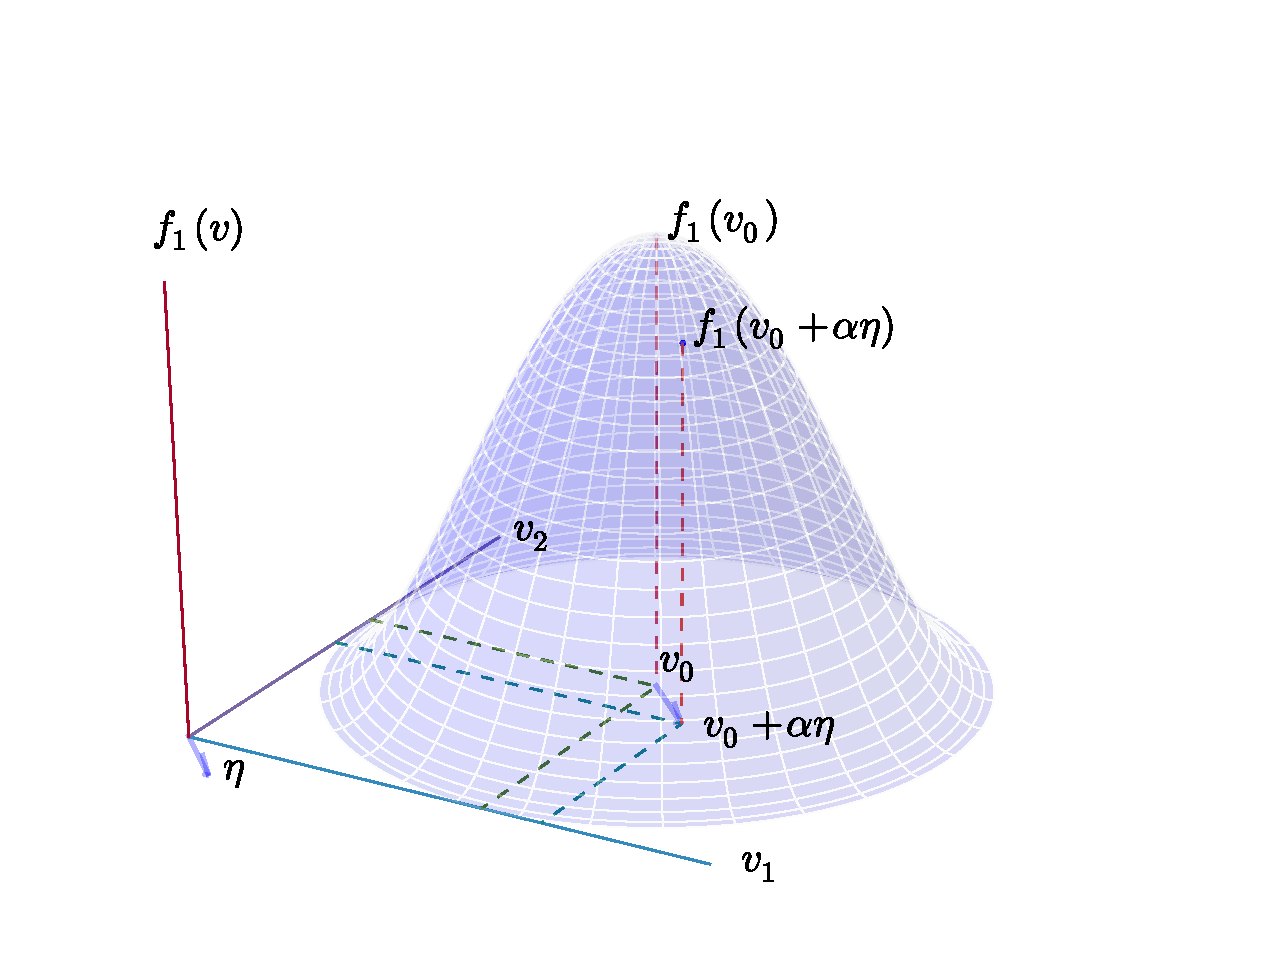
\includegraphics[width=\textwidth]{./imagenes/superficie3d.pdf}
                    \caption{\label{fig:superficie3d}Superficie de funcional con puntos a acercar.}
                \end{marginfigure}

                \begin{teorema}
                    Si $f_1$ es una función diferenciable de $v \in \mathbbm{R}^n$, entonces $f_1$ tiene una derivada direccional en la dirección de cualquier vector unitario $\eta \in \mathbbm{R}^n$ y por lo tanto:

                    \begin{equation}
                        D_{\eta} f_1(v) = \sum_{i=1}^n \frac{\partial f_1(v_i)}{dv_i} \eta_i
                    \end{equation}

                    donde $v = \begin{pmatrix} v_1 \\ v_2 \\ \vdots \\ v_n \end{pmatrix} \in \mathbbm{R}^n$, $\eta = \begin{pmatrix} \eta_1 \\ \eta_2 \\ \vdots \\ \eta_n \end{pmatrix} \in \mathbbm{R}^n$ con $|| \eta || = 1$.
                \end{teorema}

                \begin{marginfigure}
                    \centering
                    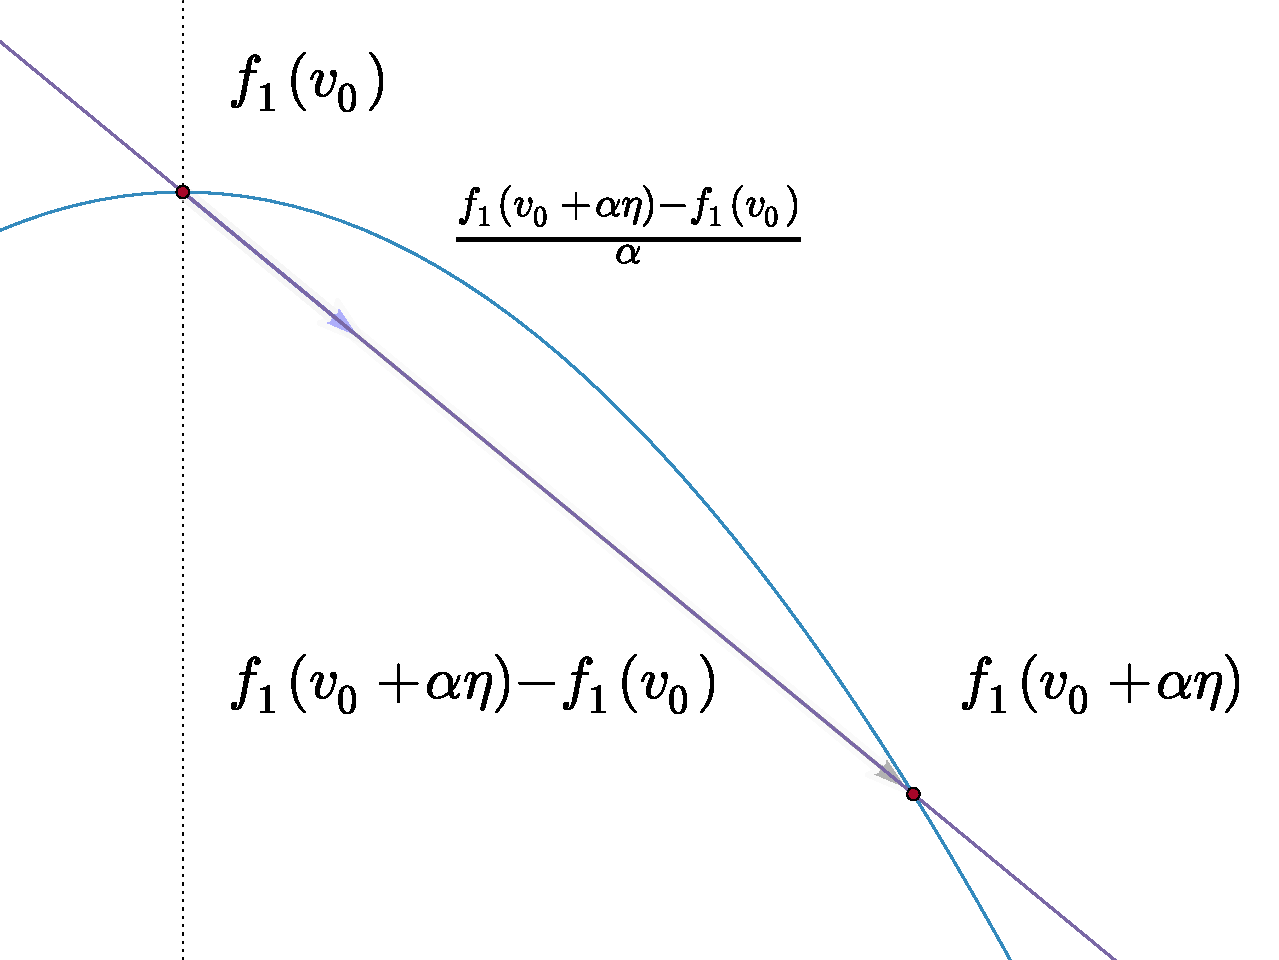
\includegraphics[width=\textwidth]{./imagenes/trayectoriaderivada.pdf}
                    \caption{\label{fig:trayderivada}Vector direccional a la derivada del funcional.}
                \end{marginfigure}

                \begin{definicion}
                    Dada una base ortonormal de $\mathbbm{R}^n$, $\left\{ e_1, e_2, \dots, e_n \right\}$, entonces el gradiente de $t_1$ es la función vectorial, $\nabla f_1$, definida por:

                    \begin{equation} \label{eq:opfun3}
                        \nabla_v f_1(v) = \sum_{i=1}^n \frac{\partial f_1}{\partial v_i} e_i
                    \end{equation}

                    donde $v_i = \sum_{i=1}^n v_i e_i$.
                \end{definicion}

                Con esta notación gradiente, la ecuación~\ref{eq:opfun3} de la derivada direccional se escribe:

                \begin{equation}
                    D_{\eta} f_1(v) = \left( \nabla f_1(v), \eta \right)
                \end{equation}

                donde $\left( R, S \right): \mathbbm{R}^n \times \mathbbm{R}^n \to \mathbbm{R}$ es el producto punto, es decir, la proyección escalar del vector $R$ sobre la dirección del vector $S$.

                \begin{teorema}
                    Suponga que $f_1: \mathbbm{R}^n \to \mathbbm{R}$ es una funcional diferenciable. El máximo valor de la derivada $D_{\eta}f(v)$ es $||D_{\eta}f(v)||$ y se obtiene cuando la dirección de $\eta$ coincide con el vector gradiente $\nabla_v f_1(v)$.
                \end{teorema}

                Sea la superficie, $\mathscr{S}$, definida por la funcional $\mathscr{G}:\mathbbm{R}^n \to \mathbbm{R}$ de la siguiente manera:

                \begin{equation}
                    \mathscr{S} = \left\{ v \in \mathbbm{R}^n \mid \mathscr{G}(v) = k \right\}
                \end{equation}

                Sea $\mathscr{C}$ una curva contenida en $\mathscr{S}$ y que pase por el punto $v_0 \in \mathbbm{R}$, la cual está definida por la función vectorial $R: \mathbbm{R} \to \mathbbm{R}^n$, esto es:

                \begin{equation}
                    \mathscr{C} = \left\{ v \in \mathbbm{R}^n, t \in \mathbbm{R} \mid v = R(t)\right\}
                \end{equation}

                Sea $t_0 \in \mathbbm{R}$ tal que $R(t_0) = v_0$.

                Como $\mathscr{C} \subset \mathscr{S}$, entonces cualquier punto, $v \in \mathscr{C}$, satisface:

                \begin{equation*}
                    \mathscr{G}(v) = k
                \end{equation*}

                lo cual implica (asumiendo que $v$ es una función diferenciable y que tambien $\mathscr{G}$ lo es):

                \begin{equation*}
                    \sum_{i=1}^n \frac{\partial \mathscr{G}}{\partial v_i} \frac{d v_i}{dt} = 0
                \end{equation*}

                es decir:

                \begin{equation*}
                    \left( \nabla_i \mathscr{G}, R'(t) \right) = 0
                \end{equation*}

                donde $R'(t) = \frac{dR(t)}{dt} = \begin{pmatrix} \frac{d v_1(t)}{dt} \\ \frac{d v_2(t)}{dt} \\ \vdots \\ \frac{d v_n(t)}{dt} \end{pmatrix} \in \mathbbm{R}^n$.

                En particular, cuando $t = t_0$, se tiene:

                \begin{equation*}
                    R(t_0) = v_0
                \end{equation*}

                \begin{equation*}
                    \left( \nabla_v \mathscr{G}(v_0), \frac{dR(t_0)}{dt} \right) = 0
                \end{equation*}

                \begin{marginfigure}
                    \centering
                    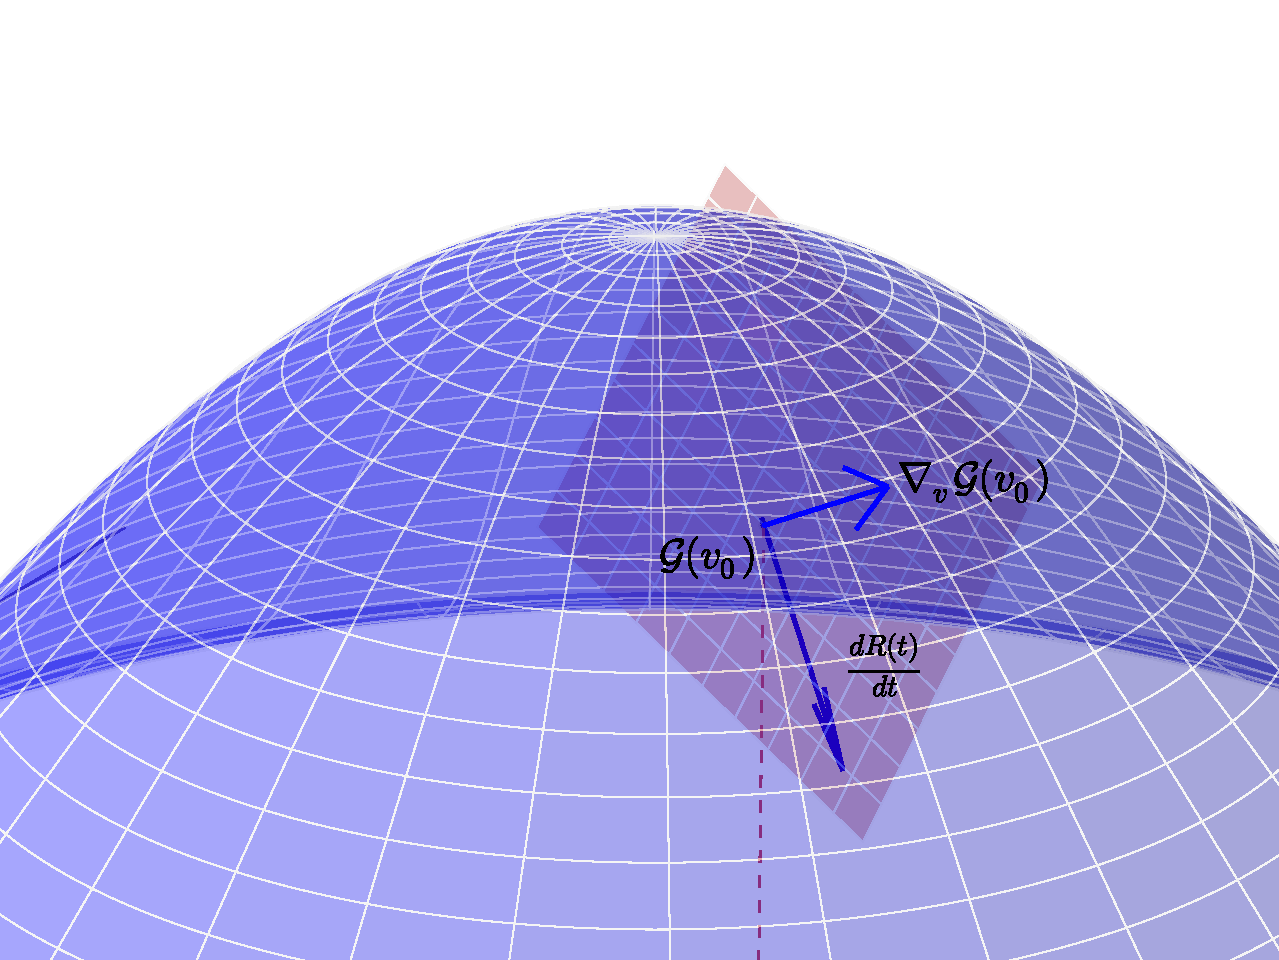
\includegraphics[width=\textwidth]{./imagenes/superficie3dplano.pdf}
                    \caption{\label{fig:supplano}Plano tangente a superficie de funcional.}
                \end{marginfigure}

                Esta ecuación indica que el vector gradiente en $v_0$, $\nabla_v \mathscr{G}(v_0)$, es perpendicular al vector tangente $\frac{dR(t_0)}{dt}$ a cualquier $\mathscr{C} \subset \mathscr{S}$ que pase por $v_0$.

                Si $\nabla_v \mathscr{G}(v_0) \ne 0$, entonces se define el plano tangente a la superficie de nivel $\mathscr{S}$, en el punto $\mathscr{G}(v_0)$ y tiene un vector normal $\nabla_v \mathscr{G}(v_0)$, esto es, el plano tangente $\tau$ que esta definido por:

                \begin{equation}
                    \tau = \left\{ v \in \mathbbm{R}^n \mid \left( \nabla_v \mathscr{G}(v_0), v - v_0 \right) = 0 \right\}
                \end{equation}

%-------------------------------------------------------------------------------

        \subsection{Multiplicadores de Lagrange}

            Procederemos ahora a resolver el problema original. Suponga que la funcional $f_1$ tiene un extremo en el punto $v_0$ en la superficie:

            \begin{equation}
                \mathscr{S}_m \left\{ v \in \mathbbm{R}^n, i \in \left\{ 1, 2, \dots, m \right\} \mid \mathscr{G}(v) = 0 \right\}
            \end{equation}

            donde $\mathscr{G}(v) = \begin{pmatrix} \mathscr{G}_1(v) \\ \mathscr{G}_2(v) \\ \vdots \\ \mathscr{G}_m(v) \end{pmatrix} \in \mathbbm{R}^m$
                y $\mathscr{G}_i(v):\mathbbm{R}^n \to \mathbbm{R}$
                con $i \in \left\{ 1,2,\dots,m \right\}$.

            Sea una curva:

            \begin{equation}
                \mathscr{C} = \left\{ v\in \mathbbm{R}^n t \in \mathbbm{R} \mid v = R(t) \right\} \subset \mathscr{S}_m
            \end{equation}

            tal que $v_0 \in \mathscr{C}$.

            Sea $t_0 \in \mathbbm{R}$ el paramtero correspondiente a $v_0$, es decir $v_0 = R(t_0)$.

            La funcional compuesta:

            \begin{equation}
                \mathscr{H} = f_1(R(t))
            \end{equation}

            representa a los valores de $f$  que también está en $\mathscr{C}$.

            Como $f_1$ tiene un extremo en $v_0$, entonces $\mathscr{H}$ tiene un extremo en $t_0$, por lo que:

            \begin{equation}
                \left. \frac{d \mathscr{H}(t)}{dt} \right|_{t=t_0} = 0
            \end{equation}

            Pero si $f$ es diferenciable, se deduce por la regla de la cadena:

            \begin{equation}
                0 = \left. \frac{d}{dt} \mathscr{H} \right|_{t=t_0} = \left. \sum_{i=1}^n \frac{\partial f_1}{\partial v_i} \frac{v_i(t)}{dt} \right|_{t=t_0, v=v_0} = \left( \nabla_v f_1(v_0), \frac{d}{dt} R(t_0) \right)
            \end{equation}

            esto nos indica que el vector gradiente $\nabla_v f_1(v_0)$, es ortogonal al vector tangente, $\frac{d R(t_0)}{dt}$, para cada una de estas curvas.

            Pero sabemos que los vectores gradientes de las coordenadas, $\left( \mathscr{G}_i, \mathscr{G}_i(v_0) \right)$, son tambien ortogonales a $\frac{d R(t_0)}{dt}$, por lo que los vectores gradiente $\nabla_v f_1(v_0)$ y $\nabla_v \mathscr{G}_i(v_0)$ con $i \in \left\{ 1, 2, \dots, m \right\}$ necesariamente son paralelos.

            Entonces, si $\nabla_v \mathscr{G}_i(v_0)$ con $i \in \left\{ 1, 2, \dots, m \right\}$, existen $\lambda_1, \lambda_2, \dots, \lambda_m$, tales que:

            \begin{equation}
                \nabla_v f_1(v_0) = \sum_{i=1}^m \lambda_i \nabla_v \mathscr{G}_i(v_0)
            \end{equation}

            y al vector $\lambda = \begin{pmatrix} \lambda_1 \\ \lambda_2 \\ \vdots \\ \lambda_m \end{pmatrix} \in \mathbbm{R}^m$ se le conoce como multiplicadores de Lagrange.

            Entonces para resolver el problema original se procede como sigue:

            \begin{enumerate}
                \item Se construye la siguiente funcional aumentada:

                \begin{equation}\label{eq:opfun3}
                    f_a(v, \lambda) = f_1(v) - \left( \lambda, \mathscr{G}(v) \right)
                \end{equation}

                \item Se encuentran los puntos estacionarios de la ecuación~\ref{eq:opfun3}:

                \begin{eqnarray}\label{eq:opfun4}
                    \nabla_v f_a(v, \lambda) & = & 0 \nonumber \\
                    \nabla_\lambda f_a(v, \lambda) & = & 0
                \end{eqnarray}
            \end{enumerate}

            El par $(v_0, \lambda_0)$ que satisface la ecuación~\ref{eq:opfun4} es la solución del problema original.

            Observe que con este método, se esta transformando un problema de optimización con restricciones, en uno sin restricciones.
